% VUT FIT MITAI
% MSZ 2021/2022
% Author: Vladimir Dusek
% Login: xdusek27

%%%%%%%%%%%%%%%%%%%%%%%%%%%%%%%%%%%%%%%%%%%%%%%%%%%%%%%%%%%%%%%%%%%%%%%%%%%%%%%%

% Path to figures
\graphicspath{{tin/klasifikace_jazyku/figures}}

%%%%%%%%%%%%%%%%%%%%%%%%%%%%%%%%%%%%%%%%%%%%%%%%%%%%%%%%%%%%%%%%%%%%%%%%%%%%%%%%

\chapter{TIN~--~Klasifikace formálních jazyků (Chomského hierarchie), vlastnosti formálních jazyků a jejich rozhodnutelnost.}

% Todo:
%  - Normalni formy (Chomskeho, Greibachove), mozna az v ramci dalsich otazek

%%%%%%%%%%%%%%%%%%%%%%%%%%%%%%%%%%%%%%%%%%%%%%%%%%%%%%%%%%%%%%%%%%%%%%%%%%%%%%%%

\section{Zdroje}

\begin{compactitem}
    \item \path{tin_2021_merged.pdf}
    \item \path{TIN_2020-09-22.mp4}
    \item \path{TIN_2020-09-29.mp4}
    \item \path{TIN_2020-10-06.mp4}
    \item \path{TIN_2020-10-13.mp4}
\end{compactitem}

%%%%%%%%%%%%%%%%%%%%%%%%%%%%%%%%%%%%%%%%%%%%%%%%%%%%%%%%%%%%%%%%%%%%%%%%%%%%%%%%

\section{Úvod a kontext}

\begin{compactitem}
    \item Symbol, znak
    \item Abeceda -- Konečná množina symbolů.
    \item Řetězec
    \item Konkatenace řetězců
    \item Reverze řetězce
    \item Podřetězec
    \item Délka řetězce
    \item Formální jazyk
    \item Doplněk jazyka
    \item Konkatenace jazyků
    \item Mocnina jazyka
    \item Iterace jazyka
\end{compactitem}

%%%%%%%%%%%%%%%%%%%%%%%%%%%%%%%%%%%%%%%%%%%%%%%%%%%%%%%%%%%%%%%%%%%%%%%%%%%%%%%%

\section{Gramatiky}

\paragraph*{Gramatika} Gramatika slouží k formální specifikaci jazyků, zejména pak nekonečných jazyků. Gramatika je čtveřice $G = (N, \Sigma, P, S)$, kde \begin{compactitem}
    \item $N$ je konečná množina neterminálů (pomocné syntaktické celky);
    \item $\Sigma$ je konečná množina terminálů (symbolů), \begin{compactitem}
        \item $N \cap \Sigma = \emptyset$;
    \end{compactitem}
    \item $P$ je konečná množina pravidel, \begin{compactitem}
        \item $P \subseteq (N \cup \Sigma)^* N (N \cup \Sigma)^* \times (N \cup \Sigma)^* $;
        \item prvek $(\alpha, \beta) \in P$ zapisujeme jako $\alpha \rightarrow \beta$;
    \end{compactitem}
    \item $S$ je výchozí neterminál, \begin{compactitem}
        \item $S \in N$.
    \end{compactitem}
\end{compactitem}

\paragraph*{Přímá derivace} Nechť $G = (N, \Sigma, P, S)$ je gramatika a nechť $\lambda, \mu \in (N \cup \Sigma)^*$. Mezi řetězci $\lambda$ a $\mu$ platí binární relace $\lambda \Rightarrow \mu$, nazývaná přímá derivace, pokud můžeme vyjádřit: $$\lambda = \gamma \alpha \delta$$ $$\mu = \gamma \beta \delta$$ kde $\gamma, \delta \in (N \cup \Sigma)^*$ a $\alpha \rightarrow \beta \in P$. Říkáme, že řetězec $\mu$ lze přímo derivovat z řetězce $\lambda$ v gramatice $G$.

\paragraph*{Derivace} Nechť $G = (N, \Sigma, P, S)$ je gramatika a nechť $\lambda, \mu \in (N \cup \Sigma)^*$. Mezi řetězci $\lambda$ a $\mu$ platí binární relace $\lambda \Rightarrow^+ \mu$, nazývaná derivace, jestliže existuje posloupnost přímých derivací $v_{i-1} \Rightarrow v_i,~~~ i=1, \dots, n,~~~ n \geq 1$, taková, že platí: $$\lambda = v_0 \Rightarrow v_1 \Rightarrow \dots \Rightarrow v_{n-1} \Rightarrow v_n = \mu$$. Tuto posloupnost nazýváme derivací délky $n$. Říkáme, že řetězec $\mu$ lze derivovat z řetězce $\lambda$ v gramatice $G$. Jestliže v gramatice $G$ platí pro řetězce $\lambda$ a $\mu$ relace $\lambda \Rightarrow^+ \mu$ a nebo identita $\lambda = \mu$, pak píšeme $\lambda \Rightarrow^* \mu$.

\paragraph*{Větná forma, věta, jazyk generovaný gramatikou} Nechť $G = (N, \Sigma, P, S)$ je gramatika. Řetězec $\alpha \in (N \cup \Sigma)^*$ nazýváme větnou formou, jestliže platí $S \Rightarrow^* \alpha$, tj. řetězec $\alpha$ je generovatelný z výchozího symbolu $S$. Větná forma, které obsahuje pouze terminální symboly, se nazývá věta. Jazyk $L(G)$ generovaný gramatikou $G$, je definován množinou všech vět $$L(G) = \{ w ~|~ w \in \Sigma^* \land S \Rightarrow^+ w \}$$.

%%%%%%%%%%%%%%%%%%%%%%%%%%%%%%%%%%%%%%%%%%%%%%%%%%%%%%%%%%%%%%%%%%%%%%%%%%%%%%%%

\section{Chomského hierarchie}

Chomského hierarchie je dělení gramatik na 4 typy dle tvaru jejich přepisovacích pravidel. Dělení gramatik odpovídá i dělení jazyků -- $L_0, L_1, L_2, L_3$. Platí: $L_0 \supseteq L_1 \supseteq L_2 \supseteq L_3$. Existují i problémy, které jsou mimo $L_0$ a tím pádem je není možné algoritmicky řešit. Chomského hierarchie vymezuje popisnou a rozhodovací sílu dané třídy.

\begin{figure}[H]
    \centering
    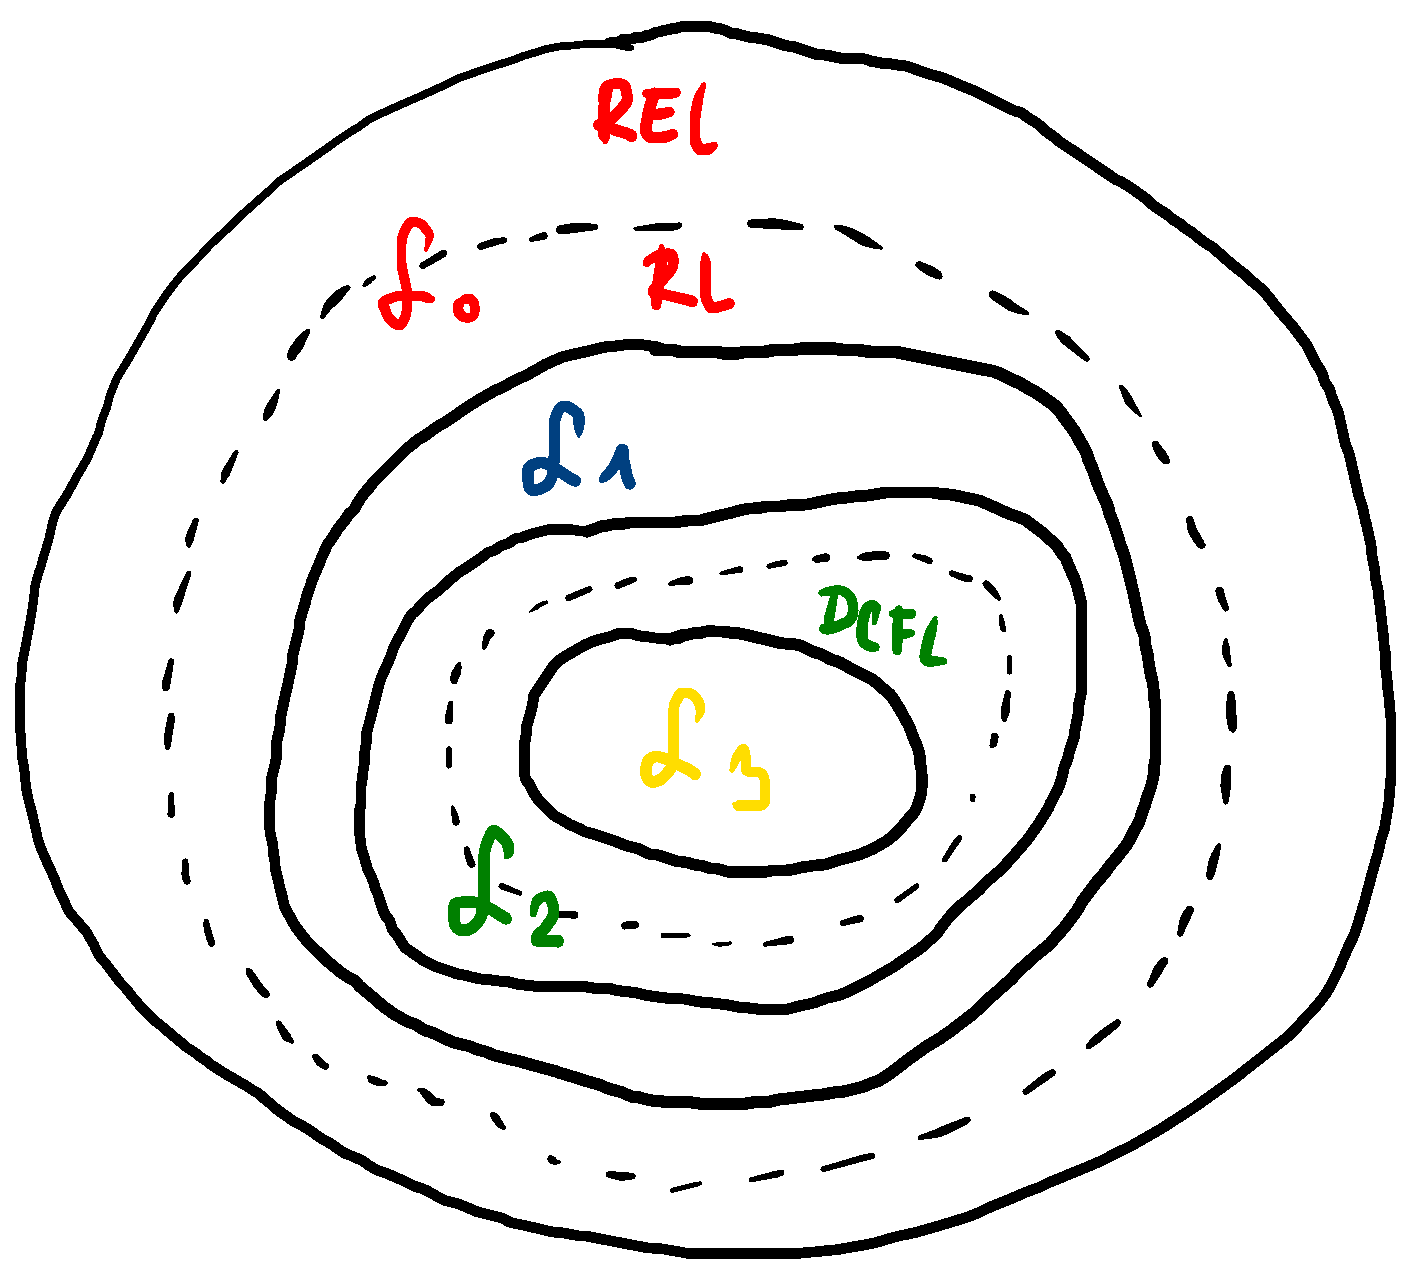
\includegraphics[width=0.6\linewidth]{chomsky_hierarchy.pdf}
    \caption{Chomského hierarchie gramatik. \textit{REL -- Recursive Enumerable Languages}, \textit{RL -- Recursive Languages}, \textit{DCFL -- Deterministic Context Free Languages}.}
\end{figure}

\paragraph*{Typ 0 (obecné / neomezené / rekurzivně vyčíslitelné gramatiky)} \begin{compactitem}
    \item Pravidla v nejobecnějším tvaru: \begin{compactitem}
        \item $\alpha \rightarrow \beta,~~~ \alpha \in (N \cup \Sigma)^* N (N \cup \Sigma)^*,~~~ \beta \in (N \cup \Sigma)^*$
    \end{compactitem}

    \item Jazyky $L_0$ jsou příjímány nedeterministickým turingovým strojem (NTS) s nekonečnou páskou.

    \item Dále existuje třída tzv. rekurzivních jazyků (RL -- \textit{Recursive Languages}). \begin{compactitem}
        \item Platí $L_0 \supset RL \supset L_1$.

        \item Jazyky $L_0$ / REL (rekurzivně vyčíslitelné jazyky) -- Turingův stroj pro ně zastaví a přijme. Jinak zastaví a nepřijme a nebo cyklí.

        \item Jazyky RL (rekurzivní jazyky) --
        Jsou přijímány úplným turingovým strojem. Ten vždy zastaví a buď přijme nebo ne, ale nemůže se zacyklit.
    \end{compactitem}
\end{compactitem}

\paragraph*{Typ 1 (kontextové gramatiky)} \begin{compactitem}
    \item Pravidla ve tvaru: \begin{compactitem}
        \item $\alpha A \beta \rightarrow \alpha \gamma \beta,~~~ A \in N,~~~ \alpha, \beta \in (N \cup \Sigma)^*,~~~ \gamma \in (N \cup \Sigma)^+$
        \item A nebo $S \rightarrow \epsilon$, pokud se $S$ nevyskytuje na pravé straně žádného pravidla (neobsahují tzv. epsilon pravidla).
    \end{compactitem}

    \item Jazyky $L_1$ jsou příjímány lineárně omezeným automatem -- nedeterministický turingův stroj (NTS) s lineárně omezenou páskou. \begin{compactitem}
        \item Omezení lineární funkcí v závislosti na délce vstupního řetězce.
        \item Z toho vyplývá, že řetězec se nemůže zkracovat, ledaže se derivuje $S \Rightarrow \epsilon$, ale v takovém případě se S nemůže vyskytovat na pravé straně žádného pravidla.
        \item Formálně: pokud $\alpha \Rightarrow \beta$, pak $|\alpha| \leq |\beta|$ (s vyjímkou $S \Rightarrow \epsilon$).
    \end{compactitem}
\end{compactitem}

\paragraph*{Typ 2 (bezkontextové gramatiky)} \begin{compactitem}
    \item Pravidla ve tvaru: \begin{compactitem}
        \item $A \rightarrow \alpha,~~~ A \in N,~~~ \alpha \in (N \cup \Sigma)^*$
        \item Mohou obsahovat i tzv. epsilon pravidla (narozdíl od kontextových).
        \item Jak je to možné, když $L_1 \supseteq L_2$?
        \item Bezkontextové gramatiky s epsilon pravidly jsou převoditelné na kontextové gramatiky bez epsilon pravidel.
    \end{compactitem}

    \item Jazyky $L_2$ jsou příjímány zásobníkovým automatem.

    \item Dále existuje třída tzv. deterministických kontextových jazyků ($L_{DCF}$ -- \textit{Deterministic Context Free Languages}). \begin{compactitem}
        \item Platí $L_2 \supset L_{DCF} \supset L_3$.
        \item Jsou přijímány deterministickým zásobníkovým automatem.
    \end{compactitem}
\end{compactitem}

\paragraph*{Typ 3 (regulární gramatiky)} \begin{compactitem}
    \item Pravidla ve tvaru: \begin{compactitem}
        \item Pravolineární: $A \rightarrow wB~|~w,~~~ A,B \in N,~~~ w \in \Sigma^*$

        \item Levolineární: $A \rightarrow Bw~|~w,~~~ A,B \in N,~~~ w \in \Sigma^*$

        \item Pravoregulární: $A \rightarrow aB~|~a,~~~ A,B \in N,~~~ a \in \Sigma$

        \item Levoregulární: $A \rightarrow Ba~|~a,~~~ A,B \in N,~~~ a \in \Sigma$
    \end{compactitem}

    \item Gramatiky se všemi tvary pravidel jsou ekvivalentní.

    \item Jazyky $L_3$ jsou příjímány konečným automatem.

    \item Každý konečný jazyk je regulární. Na konečné jazyky lze nahlížet jako na podmnožinu regulárních.
\end{compactitem}

%%%%%%%%%%%%%%%%%%%%%%%%%%%%%%%%%%%%%%%%%%%%%%%%%%%%%%%%%%%%%%%%%%%%%%%%%%%%%%%%

\section{Uzavřenost operací formálních jazyků}

\begin{compactitem}
    \item Které vlastnosti jazyků, resp. tříd jazyků, zkoumáme? \begin{compactitem}
        \item \textbf{Uzavřenost} vůči nějaké operaci -- zda výsledek operace patří do stejné třidy.

        \item \textbf{Rozhodnutelnost} problému -- zda je problém rozhodnutelný, částečně rozhodnutelný a nebo nerozhodnutelný.
    \end{compactitem}
\end{compactitem}

\paragraph*{Operace nad jazyky} \begin{compactitem}
    \item Základní množinové operace -- sjednocení, průnik, doplněk.

    \item Základní jazykové operace -- konkatenace, iterace, reverzace.

    \item Substituce -- \todo{todo}.

    \item Morfismus -- \todo{todo}.

    \item Inverzní morfismus -- \todo{todo}
\end{compactitem}

\begin{figure}[H]
    \centering
    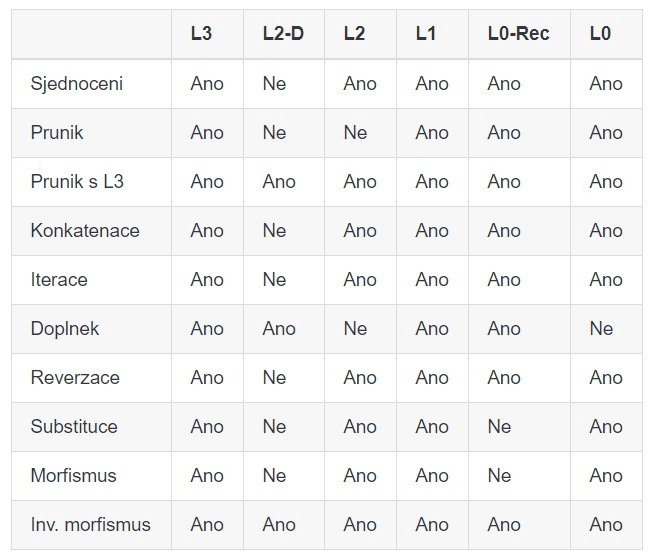
\includegraphics[width=1\linewidth]{uzavrenost_jazyku.png}
    \caption{Uzavřenost jednotlivých tříd jazyků vůči operacím.}
\end{figure}

\subsection{Uzávěrové vlastnosti regulárních jazyků}

\paragraph*{Sjednocení, průnik, doplněk, iterace, konkatenace} \begin{compactitem}
    \item Uzavřenost regulárních jazyků vůči operacím sjednocení, průnik, doplněk, iterace a konkatenace vyplývá z definice regulárních výrazů, resp. regulárních množin a ekvivalence regulárních množin a regulárních jazyků (\textit{viz otázka regulární výrazy}). \begin{compactitem}
        \item Alternativně např. pro sjednocení (pro ostatní operace je to analogické). Mějme regulární jazyky $L_1$ a $L_2$. Pak musí existovat KA $M_1$ a $M_2$, které je přijímají. Pokud jazyk $L_3 = L_1 \cup L_2$ je regulární, pak musí existovat KA $M_3 = M_1 \cup M_2$, který ho přijímá. % todo, toto neni presny
    \end{compactitem}
\end{compactitem}

\paragraph*{Doplněk ($co$)} Nechť $L \subseteq \Sigma^*$ je regulární jazyk. Nechť $M = (Q, \Sigma, \delta, q_0, F)$ je úplně definovaný KA, pro který platí $L = M(L)$. Pak KA $M' = (Q, \Sigma, \delta, q_0, Q - F)$ zřejmě přijímá jazyk $L_{co} = \Sigma^* - L$, tj. doplněk jazyka $L$.

\todo{todo: ke všemu důkazy a nebo protipříklady}

%%%%%%%%%%%%%%%%%%%%%%%%%%%%%%%%%%%%%%%%%%%%%%%%%%%%%%%%%%%%%%%%%%%%%%%%%%%%%%%%

\section{Rozhodnutelnost problémů formálních jazyků}

\paragraph*{Problémy nad jazyky} \begin{compactitem}
    \item Neprázdnost jazyka -- Jazyk je neprázdný, pokud obsahuje aspoň 1 řetězec.

    \item Prázdnost jazyka -- Jazyk je prázdný, pokud neobsahuje žádný řetězec.

    \item Konečnost jazyka -- Jazyk je konečný, pokud obsahuje konečný počet řetězců.

    \item Náležitost řetězce -- Řetězec náleží jazyku, pokud je jeho součástí.

    \item Univerzalita -- Jazyk obsahuje všechny řetězce nad abecedou ($L = \Sigma^* $).

    \item Inkluze jazyků -- Jazyk $L_1$ je inkluzí jazyka $L_2$, pokud je jazyk $L_1$ podmnožinou jazyka $L_2$.

    \item Ekvivalence gramatik -- Gramatiky $G_1$ a $G_2$ jsou ekvivalentní, pokud platí, že\break $L(G_1) = L(G_2)$. $G_1$ a $G_2$ mohou být různé.
\end{compactitem}

\begin{figure}[H]
    \centering
    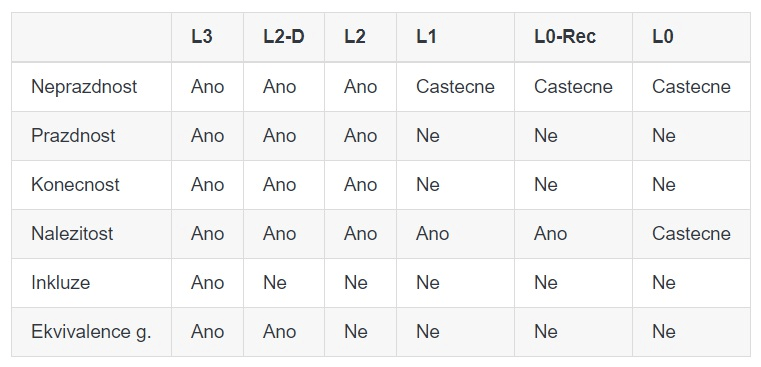
\includegraphics[width=1\linewidth]{rozhodnutelnost_jazyku.png}
    \caption{Rozhodnutelnost problémů v jednotlivých třídách jazyků.}
\end{figure}

\subsection{Rozhodnutelnost problémů regulárních jazyků}

\paragraph*{Prázdnost/neprázdnost} Problém je rozhodnutelný. Můžu sestrojit algoritmus, který pro $\forall w \in \Sigma^*$ zkusí, zda řetězec je přijímaný konečným automatem nebo není (problém dosažitelnosti konečného stavu z vychozího v grafu). Formálně: K jazyku $L \in \mathcal{L}_3$ sestrojíme úplně definovaný DKA $M$, takový, že $L = L(M)$, pak $$ L(M) \not= \emptyset \Leftrightarrow \exists q \in Q ~:~ (q \in F \land \text{q je dosažitelný z } q_0)$$

\paragraph*{Univerzalita} Problém je rozhodnutelný. K jazyku $L \in \mathcal{L}_3$ sestrojíme úplně definovaný DKA $M$, takový, že $L = L(M)$, pak $$ L(M) = \Sigma^* \Leftrightarrow \forall q \in Q ~:~ (q \in F ~\lor~ q \text{ je nedosažitelný z } q_0 )$$

\paragraph*{Náležitost} Problém je rozhodnutelný. K jazyku $L \in \mathcal{L}_3$ sestrojíme úplně definovaný DKA $M$, takový, že $L = L(M)$, pak $$ w \in L \Leftrightarrow (q_0, w) \vdash^* (q, \epsilon) \land q \in F $$

\paragraph*{Ekvivalence jazyků} Problém je rozhodnutelný. K jazyku $L_1, L_2 \in \mathcal{L}_3$ sestrojíme úplně definovaný DKA $M_1, M_2$, takový, že $L_1 = L(M_1)$ a $L_2 = L(M_2)$. Automaty $M_1, M_2$ minimalizujeme a porovnáme jejich struktury (ignorujeme identifikátory stavů).

\todo{todo: ke všemu důkazy a nebo protipříklady}
